\documentclass[spanish]{article}

\usepackage{amssymb}
\usepackage{amsmath}
\usepackage{amsfonts}
\usepackage{babel}
\usepackage[utf8]{inputenc}
\usepackage[hmargin=1cm,vmargin=1.5cm]{geometry}

\title{The Agile Unified Process (AUP)}
\date{\today}

\begin{document}
\maketitle\thispagestyle{empty}

\section{Overview}

Agile Unified Process (AUP) is a simplified version of the Rational Unified Process (RUP).
It describes a simple, easy to understand approach to developing business application software using agile techniques and concepts yet still remaining true to the RUP.
I've tried to keep the Agile UP as simple as possible, both in its approach and in its description.
The descriptions are simple and to the point, with links to details (on the web) if you want them.
The approach applies agile techniques include test driven development (TDD), Agile Model Driven Development (AMDD), agile change management, and database refactoring to improve your productivity.

Figure 1 depicts the lifecycle of the AUP.
The first thing that you'll notice is that the disciplines have changed.
First, the Model discipline encompasses the RUP's Business Modeling, Requirements, and Analysis \& Design disciplines.
Model is an important part of the AUP, as you can see, but it doesn't dominate the process -- you want to stay agile by creating models and documents which are just barely good enough.
Second, the Configuration and Change Management discipline is now the Configuration Management discipline.
In agile development your change management activities are typically part of your requirements management efforts, which is part of the Model discipline.

Figure 1. The Agile Unified Process (AUP) lifecycle.

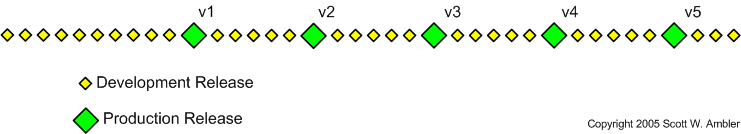
\includegraphics[scale=0.5]{incrementalReleases}


Serial in the Large

The serial nature of Agile UP is captured in its four phases :

   1. Inception. The goal is to identify the initial scope of the project, a potential architecture for your system, and to obtain initial project funding and stakeholder acceptance.
   2. Elaboration.  The goal is to prove the architecture of the system.
   3. Construction.  The goal is to build working software on a regular, incremental basis which meets the highest-priority needs of your project stakeholders.
   4. Transition.  The goal is to validate and deploy your system into your production environment.

 
Iterative in the Small

Disciplines are performed in an iterative manner, defining the activities which development team members perform to build, validate, and deliver working software which meets the needs of their stakeholders. The disciplines are:

    * Model.  The goal of this discipline is to understand the business of the organization, the problem domain being addressed by the project, and to identify a viable solution to address the problem domain.
    * Implementation.  The goal of this discipline is to transform your model(s) into executable code and to perform a basic level of testing, in particular unit testing.
    * Test.  The goal of this discipline is to perform an objective evaluation to ensure quality. This includes finding defects, validating that the system works as designed, and verifying that the requirements are met.
    * Deployment.  The goal of this discipline is to plan for the delivery of the system and to execute the plan to make the system available to end users.
    * Configuration Management.  The goal of this discipline is to manage access to your project artifacts. This includes not only tracking artifact versions over time but also controlling and managing changes to them.
    * Project Management.  The goal of this discipline is to direct the activities that takes place on the project. This includes managing risks, directing people (assigning tasks, tracking progress, etc.), and coordinating with people and systems outside the scope of the project to be sure that it is delivered on time and within budget.
    * Environment. The goal of this discipline is to support the rest of the effort by ensuring that the proper process, guidance (standards and guidelines), and tools (hardware, software, etc.) are available for the team as needed.

 
Delivering Incremental Releases Over Time

Instead of the "big bang" approach where you deliver software all at once you instead release it into production in portions (e.g. version 1, then version 2, and so on).  AUP teams typically deliver development releases at the end of each iteration into pre-production staging area(s).  A development release of an application is something that could potentially be released into production if it were to be put through your pre-production quality assurance (QA), testing, and deployment processes.  In Figure 2 you see that the first production release often takes longer to deliver than subsequent releases; in the first release of a system you likely need to get a lot of the “plumbing” in place and your team likely hasn’t “gelled” yet enabling them to become efficient at collaboration.  The first production release may take you twelve months to deliver, the second release nine months, and then other releases are delivered every six months.  An early focus on deployment issues not only enables you to avoid problems it also allows you to take advantage of your experiences during development.  For example, when you are deploying software into your staging area you should take notes of what works and what doesn’t, notes that can serve as the backbone of your installation scripts.

Figure 2. Incremental releases over time.
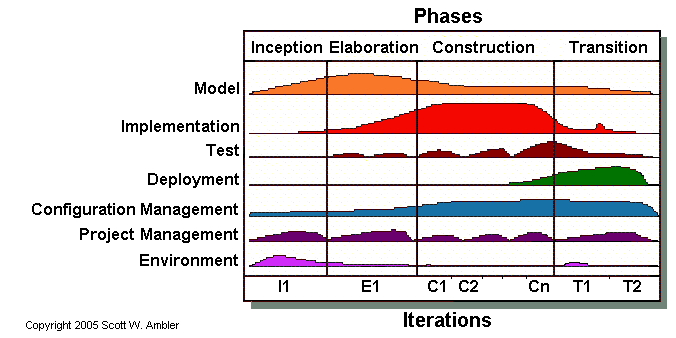
\includegraphics[scale=0.5]{lifecycleAgileUP}

Philosophies of the AUP

The Agile UP is based on the following principles:

   1. Your staff knows what they're doing.  People aren't going to read detailed process documentation, but they will want some high-level guidance and/or training from time to time.  The AUP product provides links to many of the details, if you're interested, but doesn't force them upon you.
   2. Simplicity.  Everything is described concisely using a handful of pages, not thousands of them.
   3. Agility.  The Agile UP conforms to the values and principles of the Agile Alliance.
   4. Focus on high-value activities.  The focus is on the activities which actually count, not every possible thing that could happen to you on a project.
   5. Tool independence.  You can use any toolset that you want with the Agile UP.  My suggestion is that you use the tools which are best suited for the job, which are often simple tools or even open source tools.
   6. You'll want to tailor this product to meet your own needs.  The AUP product is easily tailorable via any common HTML editing tool.  You don't need to purchase a special tool, or take a course, to tailor the AUP.

 
Some History

I first wrote about how to improve the RUP in the pages of Software Development in mid 1999.  Most of my RUP work focused on extending it via the Enterprise Unified ProcessTM (EUP) to describe how to turn the RUP into a full-fledged IT lifecycle.  In parallel, starting in early 2001, I started writing about how to "agilize" the RUP through my writings on the web and in my Agile Modeling book published in the Spring of 2002.  Since then others, in particular Craig Larman, Gary Evans, Sinan Si Alhir, and the RUP team at IBM Rational, have also written about their experiences doing so.  Object Mentor even developed an "XP plug in" for the RUP to make it look as much like XP as possible.  In September 2005 I released the first version of the AUP product at this site.  Visit here for a detailed History of the Unified Process.

 
Should You Adopt the AUP?

If you want something in between XP and traditional RUP, a process that is agile yet explicitly includes activities and artifacts which you're accustomed to, then the AUP is likely for you.  Many organizations are leery of XP because it seems to be too light: XP doesn't explicitly show how to create some of the artifacts which management wants to see.  This is an unfortunate attitude because XP is a great process.  On the other end of the spectrum is RUP, which management seems to love but developers seems leery of due to the large number of artifacts.  This is also unfortunate because the RUP has a lot to offer, and can be cut down to something quite useful (which is exactly what IBM Rational recommends you do).  The AUP lands between the two, adopting many of the agile techniques of XP and other agile processes yet retaining some of the formality of the RUP. 

The AUP isn't for everyone. The AUP is either the best of both worlds or the worst of both worlds, you be the judge.  Extreme Programmers will likely find the AUP fairly heavy, and "traditional RUP" users may find that it's too streamlined.  If you want something lighter, then I highly suggest XP.  If you want a detailed, well-defined software process then I highly suggest that you consider licensing the RUP product from IBM Rational.  


\end{document}


